\hypertarget{menu-and-action}{%
\section{Menu and action}\label{menu-and-action}}

\hypertarget{menu}{%
\subsection{Menu}\label{menu}}

Users often use menus to tell a command to the computer. It is like
this:

\begin{figure}
\centering
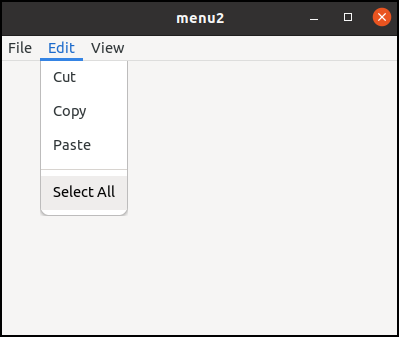
\includegraphics[width=5.985cm,height=5.055cm]{../image/menu.png}
\caption{Menu}
\end{figure}

Now let's analyze the menu above. There are two types of object.

\begin{itemize}
\tightlist
\item
  ``File'', ``Edit'', ``View'', ``Cut'', ``Copy'', ``Paste'' and
  ``Select All''. They are called ``menu item'' or simply ``item''. When
  the user clicks one of these items, then something will happen.
\item
  Menubar, submenu referenced by ``Edit'' item and two sections. They
  are called ``menu''. Menu is an ordered list of items. They are
  similar to arrays.
\end{itemize}

\begin{figure}
\centering
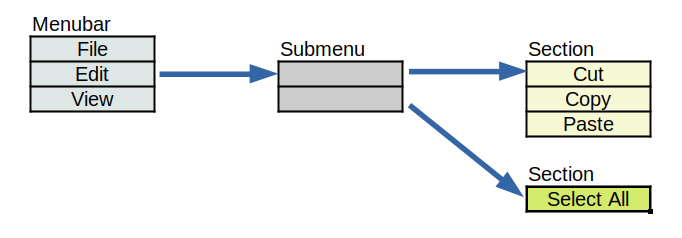
\includegraphics[width=10.23cm,height=3.57cm]{../image/menu_structure.png}
\caption{Menu structure}
\end{figure}

\begin{itemize}
\tightlist
\item
  Menubar is a menu which has three items, which are ``File'', ``Edit''
  and ``View''.
\item
  The menu item labeled ``Edit'' has a link to the submenu which has two
  items. These two items don't have labels. Each item refers to a
  section.
\item
  The first section is a menu which has three items -- ``Cut'', ``Copy''
  and ``Paste''.
\item
  The second section is a menu which has one item -- ``Select All''.
\end{itemize}

Menus can build a complicated structure thanks to the links of menu
items.

\hypertarget{gmenumodel-gmenu-and-gmenuitem}{%
\subsection{GMenuModel, GMenu and
GMenuItem}\label{gmenumodel-gmenu-and-gmenuitem}}

GMenuModel is an abstract object which represents a menu. GMenu is a
simple implementation of GMenuModel and a child object of GMenuModel.

\begin{lstlisting}
GObject -- GMenuModel -- GMenu
\end{lstlisting}

Because GMenuModel is an abstract object, it isn't instantiatable.
Therefore, it doesn't have any functions to create its instance. If you
want to create a menu, use \passthrough{\lstinline!g\_menu\_new!} to
create a GMenu instance. GMenu inherits all the functions of GMenuModel
because of the child object.

GMenuItem is an object directly derived from GObject. GMenuItem and
Gmenu (or GMenuModel) don't have a parent-child relationship.

\begin{lstlisting}
GObject -- GMenuModel -- GMenu
GObject -- GMenuItem
\end{lstlisting}

GMenuItem has attributes. One of the attributes is label. For example,
there is a menu item which has ``Edit'' label in the first diagram in
this section. ``Cut'', ``Copy'', ``Paste'' and ``Select All'' are also
the labels of the menu items. Other attributes will be explained later.

Some menu items have a link to another GMenu. There are two types of
links, submenu and section.

GMenuItem can be inserted, appended or prepended to GMenu. When it is
inserted, all of the attributes and link values of the item are copied
and used to form a new item within the menu. The GMenuItem itself is not
really inserted. Therefore, after the insertion, GMenuItem is useless
and it should be freed. The same goes for appending or prepending.

The following code shows how to append GMenuItem to GMenu.

\begin{lstlisting}
GMenu *menu = g_menu_new ();
GMenuItem *menu_item_quit = g_menu_item_new ("Quit", "app.quit");
g_menu_append_item (menu, menu_item_quit);
g_object_unref (menu_item_quit);
\end{lstlisting}

\hypertarget{menu-and-action-1}{%
\subsection{Menu and action}\label{menu-and-action-1}}

One of the attributes of menu items is an action. This attribute points
an action object.

There are two action objects, GSimpleAction and GPropertyAction.
GSimpleAction is often used. And it is used with a menu item. Only
GSimpleAction is described in this section.

An action corresponds to a menu item will be activated when the menu
item is clicked. Then the action emits an activate signal.

\begin{enumerate}
\def\labelenumi{\arabic{enumi}.}
\tightlist
\item
  menu item is clicked.
\item
  The corresponding action is activated.
\item
  The action emits a signal.
\item
  The connected handler is invoked.
\end{enumerate}

The following code is an example.

\begin{lstlisting}[language=C]
static void
quit_activated(GSimpleAction *action, GVariant *parameter, gpointer app) { ... ... ...}

GSimpleAction *act_quit = g_simple_action_new ("quit", NULL);
g_action_map_add_action (G_ACTION_MAP (app), G_ACTION (act_quit));
g_signal_connect (act_quit, "activate", G_CALLBACK (quit_activated), app);
GMenuItem *menu_item_quit = g_menu_item_new ("Quit", "app.quit");
\end{lstlisting}

\begin{enumerate}
\def\labelenumi{\arabic{enumi}.}
\tightlist
\item
  \passthrough{\lstinline!menu\_item\_quit!} is a menu item. It has a
  label ``Quit'' and is connected to an action ``app.quit''. ``app'' is
  a prefix and ``quit'' is a name of the action. The prefix ``app''
  means that the action belongs to a GtkApplication instance. If the
  menu is clicked, then the corresponding action ``quit'' which belongs
  to the GtkApplication will be activated.
\item
  \passthrough{\lstinline!act\_quit!} is an action. It has a name
  ``quit''. The function
  \passthrough{\lstinline!g\_simple\_action\_new!} creates a stateless
  action. So, \passthrough{\lstinline!act\_quit!} is stateless. The
  meaning of stateless will be explained later. The argument
  \passthrough{\lstinline!NULL!} means that the action doesn't have an
  parameter. Most of the actions are stateless and have no parameter.
\item
  The action \passthrough{\lstinline!act\_quit!} is added to the
  GtkApplication instance with
  \passthrough{\lstinline!g\_action\_map\_add\_action!}. When
  \passthrough{\lstinline!act\_quit!} is activated, it will emit
  ``activate'' signal.
\item
  ``activate'' signal of the action is connected to the handler
  \passthrough{\lstinline!quit\_activated!}. So, if the action is
  activated, the handler will be invoked.
\end{enumerate}

\hypertarget{simple-example}{%
\subsection{Simple example}\label{simple-example}}

The following is a simple example of menus and actions.

\begin{lstlisting}[language=C, numbers=left]
#include <gtk/gtk.h>

static void
quit_activated(GSimpleAction *action, GVariant *parameter, gpointer user_data) {
  GApplication *app = G_APPLICATION (user_data);

  g_application_quit (app);
}

static void
app_activate (GApplication *app, gpointer user_data) {
  GtkWidget *win = gtk_application_window_new (GTK_APPLICATION (app));
  gtk_window_set_title (GTK_WINDOW (win), "menu1");
  gtk_window_set_default_size (GTK_WINDOW (win), 400, 300);

  GSimpleAction *act_quit = g_simple_action_new ("quit", NULL);
  g_action_map_add_action (G_ACTION_MAP (app), G_ACTION (act_quit));
  g_signal_connect (act_quit, "activate", G_CALLBACK (quit_activated), app);

  GMenu *menubar = g_menu_new ();
  GMenuItem *menu_item_menu = g_menu_item_new ("Menu", NULL);
  GMenu *menu = g_menu_new ();
  GMenuItem *menu_item_quit = g_menu_item_new ("Quit", "app.quit");
  g_menu_append_item (menu, menu_item_quit);
  g_object_unref (menu_item_quit);
  g_menu_item_set_submenu (menu_item_menu, G_MENU_MODEL (menu));
  g_menu_append_item (menubar, menu_item_menu);
  g_object_unref (menu_item_menu);

  gtk_application_set_menubar (GTK_APPLICATION (app), G_MENU_MODEL (menubar));
  gtk_application_window_set_show_menubar (GTK_APPLICATION_WINDOW (win), TRUE);
  gtk_window_present (GTK_WINDOW (win));
/*  gtk_widget_show (win); is also OKay instead of gtk_window_present. */
}

#define APPLICATION_ID "com.github.ToshioCP.menu1"

int
main (int argc, char **argv) {
  GtkApplication *app;
  int stat;

  app = gtk_application_new (APPLICATION_ID, G_APPLICATION_FLAGS_NONE);
  g_signal_connect (app, "activate", G_CALLBACK (app_activate), NULL);

  stat =g_application_run (G_APPLICATION (app), argc, argv);
  g_object_unref (app);
  return stat;
}
\end{lstlisting}

\begin{itemize}
\tightlist
\item
  3-8: \passthrough{\lstinline!quit\_activated!} is a handler of the
  ``activate'' signal on the action \passthrough{\lstinline!act\_quit!}.
  Handlers of the ``activate'' signal have three parameters.

  \begin{enumerate}
  \def\labelenumi{\arabic{enumi}.}
  \tightlist
  \item
    The action instance on which the signal is emitted.
  \item
    Parameter. In this example it is \passthrough{\lstinline!NULL!}
    because the second argument of
    \passthrough{\lstinline!g\_simple\_action\_new!} (line 15) is
    \passthrough{\lstinline!NULL!}. You don' t need to care about it.
  \item
    User data. It is the fourth parameter in the
    \passthrough{\lstinline!g\_signal\_connect!} (line 18) that connects
    the action and the handler.
  \end{enumerate}
\item
  7: A function \passthrough{\lstinline!g\_application\_quit!}
  immediately quits the application.
\item
  10-34: \passthrough{\lstinline!app\_activate!} is a handler of
  ``activate'' signal on the GtkApplication instance.
\item
  12-14: Creates a GtkApplicationWindow \passthrough{\lstinline!win!}.
  And sets the title and the default size.
\item
  16: Creates GSimpleAction \passthrough{\lstinline!act\_quit!}. It is
  stateless. The first argument of
  \passthrough{\lstinline!g\_simple\_action\_new!} is a name of the
  action and the second argument is a parameter. If you don't need the
  parameter, pass \passthrough{\lstinline!NULL!}. Therefore,
  \passthrough{\lstinline!act\_quit!} has a name ``quit'' and no
  parameter.
\item
  17: Adds the action to GtkApplication \passthrough{\lstinline!app!}.
  GtkApplication implements an interface GActionMap and GActionGroup.
  GtkApplication (GActionMap) can have a group of actions and the
  actions are added with the function
  \passthrough{\lstinline!g\_action\_map\_add\_action!}. This function
  is described in
  \href{https://docs.gtk.org/gio/method.ActionMap.add_action.html}{Gio
  API Reference, g\_action\_map\_add\_action}.
\item
  18: Connects ``activate'' signal of the action and the handler
  \passthrough{\lstinline!quit\_activated!}.
\item
  20-23: Creates GMenu and GMenuItem instances.
  \passthrough{\lstinline!menubar!} and \passthrough{\lstinline!menu!}
  are GMenu. \passthrough{\lstinline!menu\_item\_menu!} and
  \passthrough{\lstinline!menu\_item\_quit!} are GMenuItem.
  \passthrough{\lstinline!menu\_item\_menu!} has a label ``Menu'' and no
  action. \passthrough{\lstinline!menu\_item\_quit!} has a label
  ``Quit'' and an action ``app.quit''. The action ``app.quit'' is a
  combination of ``app'' and ``quit''. ``app'' is a prefix and it means
  that the action belongs to GtkApplication. ``quit'' is the name of the
  action. Therefore, ``app.quit'' points the action which belongs to the
  GtkApplication instance and is named ``quit''.
\item
  24-25: Appends \passthrough{\lstinline!menu\_item\_quit!} to
  \passthrough{\lstinline!menu!}. As I mentioned before, all the
  attributes and links are copied and used to form a new item in
  \passthrough{\lstinline!menu!}. Therefore after the appending,
  \passthrough{\lstinline!menu\_item\_quit!} is no longer needed. It is
  freed by \passthrough{\lstinline!g\_object\_unref!}.
\item
  26: Sets the submenu link in
  \passthrough{\lstinline!menu\_item\_menu!} to point
  \passthrough{\lstinline!menu!}.
\item
  27-28: Appends \passthrough{\lstinline!menu\_item\_menu!} to
  \passthrough{\lstinline!menubar!}. Then frees
  \passthrough{\lstinline!menu\_item\_menu!}. GMenu and GMenuItem are
  connected and finally a menu is made up. The structure of the menu is
  shown in the diagram below.
\item
  30: The menu is inserted to GtkApplication.
\item
  31: Sets GtkApplicationWindow to show the menubar.
\item
  32: Shows the window.
\end{itemize}

\begin{figure}
\centering
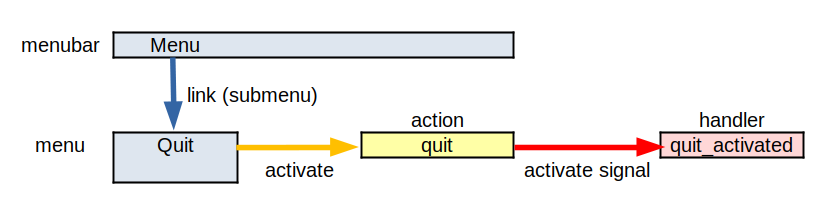
\includegraphics[width=12.555cm,height=3.285cm]{../image/menu1.png}
\caption{menu and action}
\end{figure}

\begin{figure}
\centering
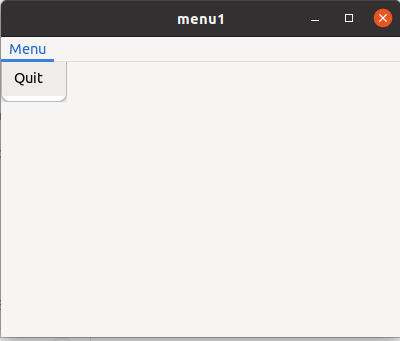
\includegraphics[width=6cm,height=5.115cm]{../image/menu1_screenshot.png}
\caption{Screenshot of menu1}
\end{figure}
